\cotefile{162-5}
\scanpage{40}

On doit trouver une approximation meilleure d'un cran à la classifica
tion topologique en prenant des (2-Cat)-groupes resp. des (2-Cat)-groupes
abéliens, ou plus généralement des ``Gr-2\unsure{'}-catégories'' resp.
``G\unsure{\deleted{a}r\deleted{r}a|\deleted{r}a\deleted{a}r}b-2-catégories'' . (NB U\deleted{n}ne Grab-catégorie défi\deleted{\unsure{t|n}}nit une Grab-2catégorie
comme une catégorie définit une 2-catégorie; du point de vue semi-simplici-
al, cette opération serait analogue à celle de ``cosquélette\deleted{''} tronqué'';
Mais également une Grab-2-catégorie définie en G\unsure{\deleted{R}r|\deleted{r}R}ab-catégorie\deleted{\unsure{.}}, savoir la
catégorie des automorphismes de l'objet unité; cette \deleted{dé} opération serait
analogue à celle de ``tuage des groupes d'homotopie en dim $>1$''). Pour la
notion gro\deleted{i}ssière (Gr\deleted{\unsure{ab}} ou Grab) l'idée de ma lettre à Verdier était qu'o\unsure{n}
doit trouver la même chose que les tronqués\inserted{au cran 2}, dans la catégorie \uline{homotopique}
des H-espaces - i.e. ce qu'on d\unsure{\deleted{d}é|\deleted{é}d}duit des H-espaces par tuage des groupes
d'homotopie en dimensions $>2$.

\margin{\figure{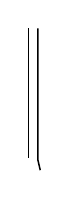
\begin{tikzpicture}[x=1cm,y=1cm,line width=.55pt]
\draw (0,0) -- (0,-1.65);
\draw (.12,0) -- (.12,-1.67) -- (.15,-1.80);
\end{tikzpicture}}}
(Demander à Quillen relations exactes entre \deleted{H}o\deleted{\unsure{-}}bjets-groupes et objets
\deleted{ponctués} connexes de la catégorie homotopique\inserted{ponctuée}: forment-ils des catégories équivalen-
tes par le foncteur espace des lacets?).
\margin{non, on a un foncteur pl. fidèle (?) mais pas \unsure{ess.$^t$|ess.} surjectif .....}

Pour les \uline{vrais} groupes\inserted{abéliens} de (2-Cat), l'approche de Quillen consiste à
les identifier \deleted{à}d'abord à des groupes abéliens de la catégorie \deleted{\unsure{d}}(Bicat),
donc à des gr\unsure{\deleted{p}o|\deleted{o}p}upes abéliens bi-semi\deleted{e}simpliciaux particuliers (\unsure{ć|c}onditions
sur chaque ligne et chaque colonne). Appliquant la version bi-semisimplici
ale du tapis de Dold, on trouve que \deleted{cette ca} la catégorie de ces objets
estb équivalente à la catégorie des \deleted{objets} bicomplexes\inserted{de chaines} de groupes abéliens
qui sont nuls en dehors du carré $\unsure{\deleted{1}0|\deleted{0}1}\leq i,j\leq1$. \deleted{Quillen dit que} La co\unsure{\deleted{o}l|\deleted{l}o}onne
que la première ligne corresponde à un \deleted{ensemble} groupe semisimplicial
trivial signifie alors qu'elle n'a que le terme de degré zéro, i.e. que
le bicomplexe est réduit à

\diagram{\begin{tikzcd}[ampersand replacement=\&,column sep=2.8em,row sep=2.2em,
execute at end picture={
\node[anchor=east,inner sep=0pt] (extraForty) at ([xshift=-.08em]lowerForty.west) {$\unsure{\deleted{0}|\theta}$};
\node[anchor=north,inner sep=0pt] (clippedForty) at ([xshift=-.65em,yshift=-.08em]lowerForty.south) {$\unsure{\pi_2}$};
\draw (extraForty.south) .. controls +(-.18,-.26) and +(-.22,0) .. (clippedForty.west);
}]
C_{oo} \& 0 \arrow[l] \& 0 \arrow[l] \\
|[alias=lowerForty]| C_{1o} \arrow[u] \& C_{11} \arrow[l] \arrow[u] \& 0 \arrow[l]
\end{tikzcd}}

\margin{39}
